%%%%%%%%%%%%%%%%%%%%%%%%%%%%%%%%%%%%%%%%%%%%%%%%%%%%%%%%%%%%%%%%%%%%%%%%%%%%%%%%
%% PIM4Agents                                                                 %%
%%%%%%%%%%%%%%%%%%%%%%%%%%%%%%%%%%%%%%%%%%%%%%%%%%%%%%%%%%%%%%%%%%%%%%%%%%%%%%%%
\section{PIM4Agents}

% PIM4Agents - references
This section introduces the PIM4Agents\footnote{For `Platform-independent model for agents'.} metamodel described in \cite{Hahn07a}, \cite{Hahn07b} and \cite{Hahn08}.
We will present only a brief overview (particularly after \cite{Hahn07b}) since our work does not draw inspiration from PIM4Agents.

% PIM4Agents - authors
PIM4Agents has been proposed in 2007 by Christian Hahn, Cristián Madrigal-Mora and Klaus Fischer from German Research Centre for Artificial Intelligence (Deutsches Forschungszentrum f\"{u}r K\"{u}nstliche Intelligenz, DFKI).

%% Summary %%%%%%%%%%%%%%%%%%%%%%%%%%%%%%%%%%%%%%%%%%%%%%%%%%%%%%%%%%%%%%%%%%%%%

- PIM

% PIM4Agents & MDA
PIM4Agents has been specifically designed to be employed in the Model-driven engineering (MDE) software development methodology, more precisely the Model-driven architecture (MDA) by Object Management Group (OMG).
Apart from the platform-independent metamodel itself, the authors have proposed two platform-specific metamodels: JackMM (for JACK) and JadeMM (for JADE).
They have also described two sets of model transformations to convert platform-independent models (PIM) to platform-specific models (PSM): PIM4Agents to JackMM and PIM4Agents to JadeMM.

%%%%%%%%%%%%%%%%%%%%%%%%%%%%%%%%%%%%%%%%%%%%%%%%%%%%%%%%%%%%%%%%%%%%%%%%%%%%%%%%
\subsection*{Core Metamodel}

% Core metamodel
In order to support an evolution, the PIM4Agents metamodel is structured around a small core that could possibly be augmented with extensions to model specific (even unforeseen) aspects of MAS, for example security.
The core metamodel is shown in figure~\ref{figure:pim4agents-metamodel}.
The metamodel, like previous metamodels, is built around the concept of \textsc{Agent}, an autonomous entity capable of sensing and acting upon its environment.
Each \textsc{Agent} has access to a set of \textsc{Resources} from its surrounding \textsc{Environment}.

\textsc{Behaviour} can be primitive (ALT: simple) or composed of sub-behaviours; a whole hierarchy of specific \textsc{Behaviours} can be created.
\textsc{Behaviour} may also send or receive a \textsc{Message} according to a given \textsc{Protocol}.
\textsc{Capability} allows to group \textsc{Behaviours} that, conceptually, have a correspondence with regard to what they allow \textsc{Agent} to do.

\textsc{Role} is an abstraction of the social behaviour of the Agent in a given social context, usually \textsc{Cooperation}.
This \textsc{Role} specifies the responsibilities of \textsc{Agent} in that social context.
Correspondingly, \textsc{Cooperation} represents the interaction between \textsc{Agents} performing the required set of \textsc{Roles}.
The detailed realisation of this interaction is described by \textsc{Protocol} that indicates what are \textsc{Messages} to be expected from each of \textsc{Roles} at which point in time.
The execution of \textsc{Protocol} is performed by a set of \textsc{Behaviours}, each of which sends and/or receives \textsc{Messages} in accordance to its \textsc{Role}.

\textsc{Agents} can take part in \textsc{Organisation}, a special kind of \textsc{Cooperation} that also has the same characteristics as \textsc{Agent}.
Therefore, \textsc{Organisation} can perform roles and has \textsc{Capabilities} which can be performed by its members, be it \textsc{Agents} or sub-organisations.
The multiple inheritance of \textsc{Organisation} from \textsc{Agent} and \textsc{Cooperation} also allows it to have its own internal protocol that specifies how \textsc{Organisation} coordinates its members.

% Figure: PIM4Agents metamodel
\begin{figure}[ht]
	\centering
	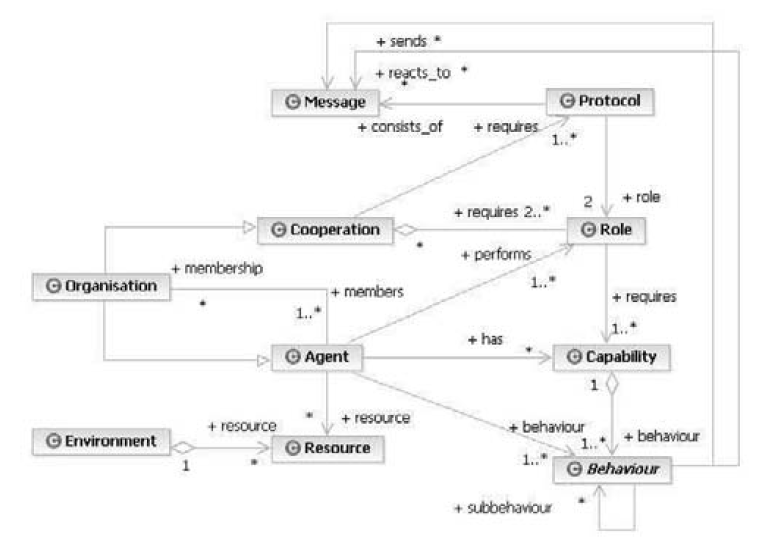
\includegraphics[width=\textwidth]{images/pim4agents-metamodel.png}
	\caption{The PIM4Agents metamodel}
	\label{figure:pim4agents-metamodel}
\end{figure}

%%%%%%%%%%%%%%%%%%%%%%%%%%%%%%%%%%%%%%%%%%%%%%%%%%%%%%%%%%%%%%%%%%%%%%%%%%%%%%%%
\subsection{JadeOrgs}

JadeOrgs is an extension of the JADE (agent?) platform that implements the JadeMM platform-specific metamodel.
JadeMM is defined using Eclipse Modeling Framework (EMF) to exploit EMF's code generation facility; given a platform-independent model of a MAS (conforming to PIM4Agents), the corresponding JADE/JadeOrgs platform-specific model (conforming to JadeMM) can be derived automatically.

JadeOrgs has been described in \cite{Madrigal-Mora08} and \cite{Madrigal-Mora09}.